%\documentclass[times, 10pt, twocolumn]{article}
%\documentclass[conference,final]{IEEEtran}

\documentclass{rspublic}

%------------------------------------------------------------------------- take
%the % away on next line to produce the final camera-ready version
%\pagestyle{empty}

\usepackage{graphicx}
\usepackage{float}
\usepackage{times}
\usepackage{multirow}
\usepackage{listings}
%\usepackage{paralist}
%\usepackage{wrapfig}
\usepackage[small,it]{caption}
\usepackage{ifpdf}
\usepackage{subfigure}
\usepackage{url}

%Bibliography
\usepackage{natbib}
\usepackage{listings}
\usepackage{keyval}
\usepackage{color}
\definecolor{listinggray}{gray}{0.95}
\definecolor{darkgray}{gray}{0.7}
\definecolor{commentgreen}{rgb}{0, 0.4, 0}
\definecolor{darkblue}{rgb}{0, 0, 0.4}
\definecolor{middleblue}{rgb}{0, 0, 0.7}
\definecolor{darkred}{rgb}{0.4, 0, 0}
\definecolor{brown}{rgb}{0.5, 0.5, 0}
\definecolor{orange}{rgb}{1,0.5,0}

\lstdefinestyle{myListing}{ frame=single, backgroundcolor=\color{listinggray},
  %float=t,
  language=C, basicstyle=\ttfamily \footnotesize, breakautoindent=true,
breaklines=true tabsize=2, captionpos=b, aboveskip=0em,
  %numbers=left, numberstyle=\tiny
}

\lstdefinestyle{myPythonListing}{ frame=single,
backgroundcolor=\color{listinggray},
  %float=t,
  language=Python, basicstyle=\ttfamily \footnotesize,
breakautoindent=true, breaklines=true tabsize=2, captionpos=b,
  %numbers=left, numberstyle=\tiny
}

\title[Understanding Performance Implications of Distributed Data for
Data-Intensive Applications]{Understanding Performance Implications of
Distributed Data for Data-Intensive Applications}

\author[Miceli, Miceli, Rodriguez-Milla, Jha]{ Christopher Miceli$^{1}$,
Michael Miceli$^{1}$, Bety Rodriguez-Milla$^{1}$, Shantenu Jha$^{1,2,*}$ \\
\small{\emph{$^{1}$Center for Computation \& Technology, Louisiana State
University, USA}} \\  \small{\emph{$^{2}$Department of Computer Science,
Louisiana State University, USA}} \\ {\footnotesize {\hspace{0.0 in}
$^*$Corresponding Author sjha@cct.lsu.edu}} }

%\date{}

\def\acknowledgementname{Acknowledgements} \newenvironment{acknowledgement} 

% {\section*{\acknowledgementname}%\parindent=0pt% }

\newif\ifdraft 
\drafttrue 
\ifdraft 

\newcommand{\fixme}[1]{ { \bf{ ***FIXME: #1
}} } \newcommand{\jhanote}[1]{ {\textcolor{red} { ***Jha: #1 }}}
\newcommand{\micnote}[1]{ {\textcolor{blue} { ***Michael: #1 }}} 
\newcommand{\betynote}[1]{ {\textcolor{orange} { ***Bety: #1 }}}
\else
\newcommand{\jhanote}[1]{} \newcommand{\micnote}[1]{}\newcommand{\betynote}[1]{} \newcommand{\fixme}[1]{}
\fi

\begin{document} \maketitle

\begin{abstract}{data-intensive computing, distributed computing,
cloud computing, grid computing} 
Grids, clouds, and cloud-like infrastructures are capable of supporting
a broad range of data-intensive applications. There are interesting
and unique performance issues that appear as the volume of data and
degree of distribution increases. New scalable data placement and
management techniques, as well as novel approaches to determine the
relative placement of data and computational workload are required. We
develop and study an All-Pairs based genome sequence matching
application as a representative data-intensive application.  This paper
aims to understand the factors that influence the performance of this
application and their interplay.  % We are not aware
% of similar approaches for data-intensive applications, even though
% analogous benchmarking HPC application on a new platform is
% established practise.  
We also demonstrate how the SAGA approach can enable data-intensive
applications to be extensible and interoperable over a range of
infrastructure. This capability enables us to compare and contrast two
different approaches -- simple application-level data placement
strategies versus distributed file systems -- for executing distributed
data-intensive applications.

% Grids, clouds and cloud-like infrastructures are capable of supporting a
% broad range of data-intensive applications. There are interesting and
% unique performance issues that appear as the volume of data increases
% which require scalable data placement and management techniques, as well
% as novel approaches to the relative placement of data and computational
% workload. This paper aims to understand the factors that determine the
% performance of a representative data-intensive application, and to
% understand the performance trade-offs in design decisions. This is
% analogous to benchmarking the performance of an application on a new
% platform. We analyse two techniques to manage data placement. One
% focuses on data placement and the other on worker placement. The goal of
% this paper is to understand techniques for distributing data in a
% distributed environment and understand performance issues associated
% with these techniques.
\end{abstract}

\vspace{-0.3cm}

\section{Introduction} 
The role of data-intensive computing is increasing in many aspects of
science and engineering~\citep{fourthparadigm} and other
disciplines. For example, Google processes around 20 petabytes of data
per day~\citep{google}, with trends showing continuing growth. In
addition to increasing volumes of data, there are several reasons
driving the need for computation on distributed data, such as the
proliferation of distributed services and the localisation of data due
to security \& privacy issues. The challenges in developing effective
and efficient distributed data-intensive applications are a complex
interplay of the challenges in developing distributed applications on
the one hand with those in developing data-intensive applications to
meet a range of design \& performance metrics in the other. New
algorithmic, infrastructure, and data-management techniques are
required to handle large data-volumes effectively. In general at such
large scales data-placement, data-scheduling, as well as management
need increased attention.

An important design consideration and objective for data-intensive
distributed applications and systems is the ability to find and
support optimal distribution of data and computational workload. Thus
an important challenge is to find broadly applicable strategies to
distribute data and computation that can support a range of different
mechanisms to achieve this objective. In general, there are many
degrees-of-freedom that determine the performance of a given
application on distributed infrastructure. Thus a rigorous
benchmarking process, which provides repeatable, extensible, and
verifiable performance tests on different distributed platforms is
required in order to understand the interplay and trade-offs between
these variables. This is analogous to the situation of developing and
testing benchmarks for high performance computing (HPC). 

The work in this paper is performed in the context of a SAGA-based
application to support genome sequence matching to determine and
analyse performance that we developed. SAGA encodes the All-Pairs
pattern in a distributed context; we chose All-Pairs as it is a
representative and common data-access pattern found in many
data-intensive distributed applications.  In this paper, we
investigate two ways to handle the optimal data-computation distribution
problem.  In the first approach, we encode a simple metric to determine
the {\it workload} placement into a ``heuristic framework''. We contrast
this approach with the use of an open-source distributed filesystem
(DFS) -- which natively supports effective {\it data} placement.  A DFS
controls the data placement and provides a uniform interface for
accessing files on multiple hosts. DFS are becoming increasing common as
part of Cloud infrastructures and available machine images. But the
underlying algorithms, scheduling strategies, and implementations vary
greatly between different infrastructure, hence it is difficult to
estimate {\it a priori} the application-level performance on a given
DFS.  Thus having the ability to compare and contrast different DFSs for
a given application is an important requirement. In Section 3 we will
establish how the use of adaptors enables SAGA-based applications to
make this comparison effectively.  An aim of this paper is to present a
credible initial benchmarking template, and to suggest ways to answer
the question of whether ``to move computational workload to where data
resides or to redistributed the data''.  As we will show, the actual
answer will depend significantly on the specific data-set sizes,
algorithm/applications, and infrastructure used.  Data privacy,
security, and access policy are crucial issues but typically are not
determinants of performance for distributed applications; thus we will
not consider them in this paper.

In Section 2, we provide a very brief discussion of SAGA which
provides the distributed programming capability to develop the
All-Pairs based application (Section 3). Section 4 provides an
overview of the various parameters used to understand the experimental
configurations, discusses the experiments carried out to understand
the performance, as well as provides a local analysis of the
experimental results. Section 5 provides an overview of our the
understanding gained and a look ahead.

% Frequently, there is more than one copy of the input data for
% fault-tolerance reasons, consequently, the added issue of deciding
% between the two or more replicas becomes relevant.

% This puts pressure on a DFS's protocols and internal algorithms to
% perform well. Despite this, the DFS replication may alleviate this
% issue by placing replicas in locations where computational resources
% reside. A downfall of DFS is the inability to make the decision of
% whether to move the input data, or the computational workload. It
% can only focus on minimizing poor data management.

\vspace{-0.3cm}

\section{SAGA and SAGA-based Frameworks for Large-Scale and
 Distributed Computation}\label{Sec:SAGA}

%\alnote{removed the first paragraph - duplicated content}
% SAGA~\cite{saga_url} provides a simple, POSIX-inspired API to the most
% commonly required distributed functionality at a sufficiently
% high-level of abstraction so as to be independent of the divers\ e and
% dynamic Grid environments.

The Simple API for Grid Applications (SAGA) is an API
% standardization effort within the Open Grid Forum
% (OGF)~\cite{saga_gfd90}, an international standards development body
% concerned primarily with standards for distributed computing. 
that provides a simple, POSIX-style API to the most common distributed
functions at a sufficiently high-level of abstraction so as to be
independent of the diverse and dynamic Grid environments. The SAGA
specification defines interfaces for the most common Grid-programming
functions grouped as a set of functional packages
(Fig.~\ref{Fig:SAGA1}). Some key packages are: (i) File package -
provides methods for accessing local and remote filesystems, browsing
directories, moving, copying, and deleting files, setting access
permissions, as well as zero-copy reading and writing. (ii) Job
package - provides methods for describing, submitting, monitoring, and
controlling local and remote jobs. Many parts of this package were
derived from the largely adopted DRMAA specification. (iii) Stream
package - provides methods for authenticated local and remote socket
connections with hooks to support authorization and encryption
schemes. (iv) Other Packages, such as the RPC (remote procedure call)
and Replica package.

\begin{figure}[!ht]
 \begin{center}
     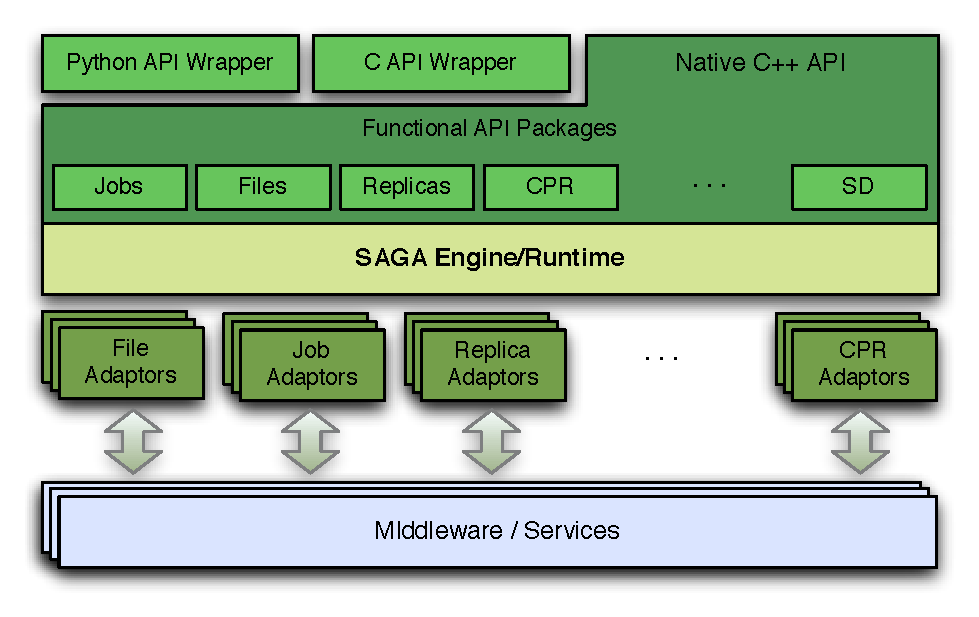
\includegraphics[width=0.47\textwidth]{stci_saga_figures-1.pdf}
    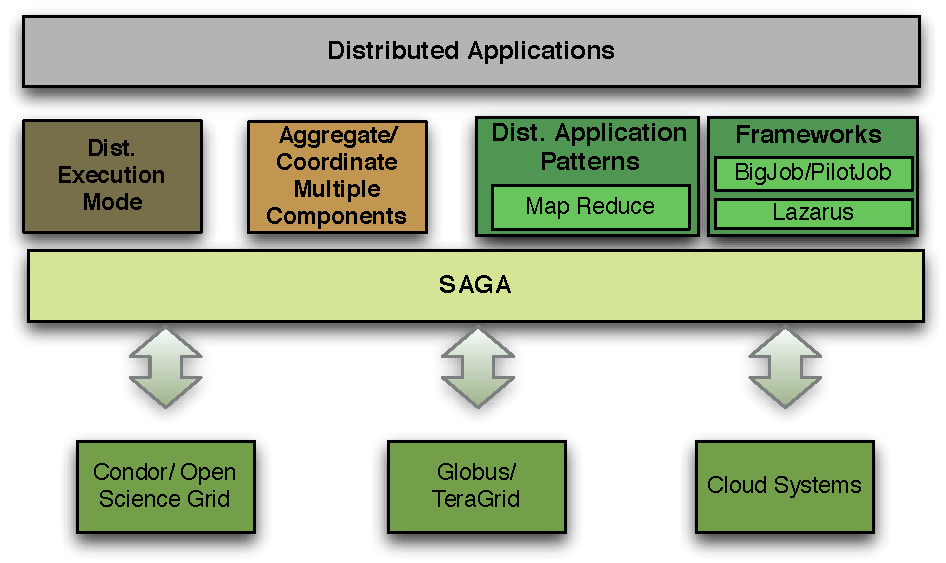
\includegraphics[width=0.48\textwidth]{distributed_applications_saga_figure.pdf}
\end{center}
\caption{\small [Left] Layered schematic of the different components
  of the SAGA landscape. At the topmost level is the simple integrated
  API which provides the basic functionality for distributed
  computing. Our BigJob abstraction is built upon this SAGA layer
  using Python API bindings. [Right] Showing the ways in which SAGA
  can be used to develop distributed applications. The different
  shaded box represent the three different types; frameworks in turn
  can capture either common patterns or common application
  requirements/characteristics.} \label{Fig:SAGA1}
\end{figure}

In the absence of a formal theoretical taxonomy of distributed
applications, Fig.~\ref{Fig:SAGA1} can act a guide. Using this
classification system, there are three types of distributed
applications: (i) Applications where local functionality is swapped
for distributed functionality, or where distributed execution modes
are provided. % A simple but illustrative example is an ensemble of an
% application that uses distributed resources for bulk submission. Here,
% the application remains unchanged and even unaware of its distributed
% execution, and the staging, coordination, and management are done by
% external tools or agents. Most application in this category are
% classified as implicitly distributed.  
(ii) Applications that are naturally decomposable or have multiple
components are then aggregated or coordinated by some unifying or
explicit mechanism. %  DAG-based workflows are probably the most common
% example of applications in this category.
Finally, (iii) applications that are developed using frameworks, where a
framework is a generic name for a development tool that supports
specific application characteristics (e.g., hierarchical job
submission), and/or recurring patterns (e.g., MapReduce, All-Pairs).
SAGA provides the basic API to implement distributed functionality
required by applications (typically used directly by the first category
of applications), and is also used to implement higher-level APIs,
abstractions, and frameworks that, in turn, support the development,
deployment, and execution of distributed
applications~\citep{saga_gmac09}. SAGA has been used to develop
system-level tools and applications of each of these types.
In~\cite{saga_montage_escience09} we discussed how SAGA was used to
implement a higher-level API to support workflows.
In~\cite{saga_ccgrid09} we discussed how a saga-based MapReduce was developed.

% In this paper, we will discuss how SAGA can be used to implement
% runtime frameworks to support the efficient execution of the
% distributed applications.

% \begin{figure}[!ht]
%   \begin{center}
%     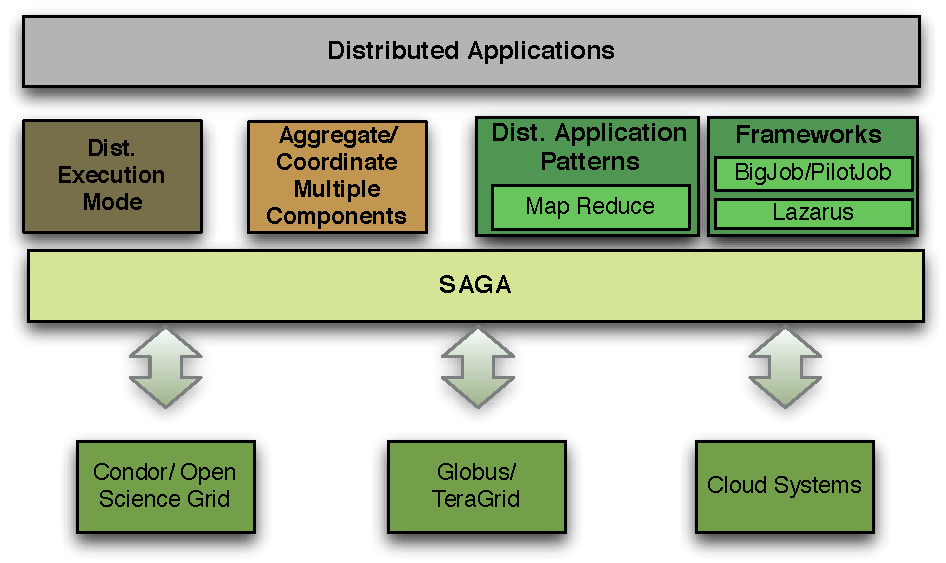
\includegraphics[width=0.45\textwidth]{distributed_applications_saga_figure.pdf}
%   \end{center}
%   \caption{\small Showing the ways in which SAGA can be used to
%     develop distributed applications.  The different shaded box
%     represent the three different types; frameworks in turn can
%     capture either common patterns or common application
%     requirements/characteristics. \label{Fig:sagaapps}}
% \end{figure}

\vspace{-0.3cm}

\section{All-Pairs: Design, Development and Infrastructure} We use an
application based upon an All-Pairs abstraction whose distributed
capabilities are developed using SAGA. The All-Pairs pattern was
chosen because of its pervasive nature and applicability to many other
data-intensive distributed applications. This enables our results to
be abstracted to describe and predict different applications in
addition to the genome sequence matching with similar structured
data-access patterns.

The All-Pairs abstraction applies an operation on two data-sets such
that every possible pair containing one element from the first set and
one element from the second set has some operation applied to
it~\citep{AllPairs}. Essentially, All-Pairs is a function of two sets,
$A$ and $B$, with number of elements $m$ and $n$, respectively, which
creates a matrix $M$. Each element $M_{i,j}$ is the result of the
operation $f$ applied to the elements $A_i$ and $B_j$.
\begin{eqnarray}
 AllPairs(A, B, f) & \rightarrow & M_{m \times n}, \\
\mbox{where} \quad M_{i,j} & = & f(A_{i},B_{j})
 \end{eqnarray}

The result of this application is stored in a matrix similar to Fig.
\ref{Fig:AllPairsExplanation}. The application spawns distributed jobs
to run sets of these function operations. Examples of problems that fall
into this category are image comparison for facial recognition, and
genome comparison.  The usefulness of All-Pairs comes from the ability
to easily change the function without whole-scale refactoring.
  We use a SAGA-based All-Pairs framework
and simply implemented the comparison function.  Our comparison function
compares genome to find the best matching gene in a genome.  The
function finds the number of similarities among the genes and returns
the percentage of the genes that are identical. Despite having a
relatively small output $O$(KB), our genome comparison application can
be classified as having a large data throughput as it has large input
$O$(GB) with many data reads.

\begin{figure}[!ht]
 \begin{center}
     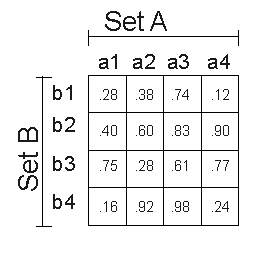
\includegraphics[width=0.3\textwidth]{data/allpairs-exp.pdf}
\end{center}
\caption{\small An example result from an All-Pairs enabled application.
Each matrix element describes the similarity between the corresponding
sets. (Larger values indicate greater similarity.)}
 \label{Fig:AllPairsExplanation}
\end{figure}

The problem becomes a two-level assignment problem: first,
which pairs to put into an assignment
set, and second, with which distributed resource to run that set.  If
transferring data to the job takes too long, we spend more time on
data transfer than computation. There may be a resource capable of the
work that may be slower than others, but able to be accessed in a
relatively quick manner via the network, correcting for this lack of
computational ability. An application can uses simple heuristics to
predict and determine a specific data set's affinity to a specific
network resource.

%\subsection{Infrastructure Used}

{\it Infrastructure Used: } In our experiments we use the stable, open-source DFS CloudStore
(formerly KFS), which is written in C++ and released under the Apache
License Version 2.0 ~\citep{cloudstore_web}. It is inspired by the highly successful Google
Filesystem, GFS, which is closed source and
unavailable for research. CloudStore was chosen for its high
performance focus, C++ implementation, and its source code
availability. It also provides a means to automatically replicate data
on different hosts to provide efficient data access and fault
tolerance. In general, DFS are useful and effective tools to consider
for data-intensive scientific applications,
with multiple open-source, reliable file-systems now available.  The
most common parameters in determining the performance of using a DFS
are the performance overhead compared to a normal local filesystem,
number of replicas of each datum/file, and the number of servers.
While a DFS removes the responsibility of replica management and data
server placement, the abstraction often increases the difficulty in
determining where in the DFS the data is being stored.

Here we define our \textit{heuristic framework} method, it differs from a DFS in that it
determines where data is located and where the work should be placed. Determining
data location can be as simple as looking at the IP address of the
worker and finding where it is located, or as
complicated as using network analysis tools to determine the optimal
data transfer minimization time. For file transfer during these
heuristic framework-based experiments, we use GridFTP -- a tool that can
support high-performance transfers ~\citep{gridftp_web}.

To test the performance of CloudStore and GridFTP, we wrote adaptors for SAGA that
implement the filesystem package. 
SAGA allows our application
to handle seamlessly the DFS and GridFTP based data stores on clouds and
grids, enabling us to compare both.
For accurate comparisons, we must consider the
overhead introduced by SAGA. We have measured a slight difference in
times; however, the adaptor implementations grew at the same rate as
GridFTP and CloudStore usage without SAGA.  

% While a DFS removes the responsibility of
% replica management and data server placement, the abstraction often
% increases the difficulty in determining where in the DFS the data is
% being stored. This puts pressure on a DFS's protocols and internal
% algorithms to perform well. Despite this, the DFS replication may
% alleviate this issue by placing replicas in locations where
% computational resources reside.
% A drawback of most DFS is their inability to
% make the decision of whether to move the input data, or the
% computational workload. It can only focus on minimizing poor data
% management. 

\vspace{-0.3cm}

\section{Experiments and Performance Analysis} 
We developed three types of experiments in order to understand the
interplay of different determinants of performance and make a
meaningful comparison of CloudStore's behaviour to manual data
placement and file management. We try to answer questions such as: Is
a DFS slower than manual placement of data?  When manually handling
data, what are the advantages of being able to move work to data, or
data to the work? To answer these questions, we define the time to completion $t_c$:
 \begin{equation}
t_c = t_x + t_{I/O} + t_{compute},
\end{equation}
where $t_x$ is the pre-processing time, the dominant component of which is
the time for transfer, $t_{I/O}$ is the time it takes to read and write
files, and $t_{compute}$ is the time it takes our comparison function to
run. We focus on three variables to calculate $t_c$: degree of
distribution, data dependency, and workload. The degree of distribution
($D_d$) is defined as the number of resources that are utilized for a
given computation/problem. For example, if data is distributed over 3
machines, $D_d=3$; if data is distributed over three machines but the
computational tasks over 4 machines, $D_d=4$.

\vspace{-0.3cm}

\subsection{Experimental Configuration}

As explained before, for our experiments, we use an All-Pairs
implementation that utilises SAGA. An XML configuration file defines
various initial parameters of the All-Pairs
implementation. The configuration file defines the location of data that
comprises the two input sets, the grouping of pairs from these sets to
be provided to the compute resources, and the available machines that
will perform the operation on these sets of pairs. The application takes
these groups of pairs and maps them to a computational resource
dynamically at run-time.

Furthermore, variables external to the All-Pairs implementation also
influence experimental results. Our experiments can be
completely described by a tuple of the following form
 \begin{equation}
(c_s, N_c, M_c, f\!s, m,r),
\label{Eq:tuple}
\end{equation}
where $c_s$ is the total amount of data in each file of a set (i.e.,
$c_s=\mbox{\textit{chunk} size}$); $N_c$ is the number of work-loads
that the total work is decomposed into, i.e., number of work assignments
generated. $M_c$ will be
represented by configurations \textit{C1, C2, C3, C4}, or \textit{C5}, each of
which is a comma separated list of the machine configurations of the
following form: $X(c, d)$ where $X$ is a shorthand reference for the
computational resource, $c$ shows if the computational resource $X$ was
used in the computational workloads/calculations, and $d$ if the
computational resource $X$ assisted in data storage, both have a yes/no
$(Y/N)$ value (see Table \ref{Tab:Configs}); $f\!s$ is the type of
filesystem used; $m$ is the method used to access that filesystem; and
$r$ is the degree of replication utilized in the experiment (with a
default value of 1).  However, for CloudStore, we investigate the
performance with $r = 1, 2
\mbox{ and } 3$.

In our experiments, we have three $(f\!s, m)$ configurations, and five
$X$ configurations. Our $(f\!s, m)$ configurations are (local, local),
(local, GridFTP), and (CloudStore, direct). By direct we mean CloudStore
controls the data access. Our $X$ configurations are enumerated in Table
\ref{Tab:Configs}. For one machine, $\textit{C1}=X_1(Y,Y)$, where resource $X_1$
has both the data and the computing; for two machines, we have three
configurations, and for three machines we only work with only one
configuration. $N_c$ is a very important configuration parameter as it
determines the granularity of work. By granularity, we mean the ability
to be distributed to many resources.  If $N_c$ is too small, there may
exist idle resources unable to assist the workload while the ones that
are participating are overloaded.

\begin{table}
\begin{center}
    \begin{tabular}{ | l | l | l |}
    \hline
    Configurations & $X(c,d)$; $c= \mbox{compute}$, $d=\mbox{data storage}$ & Description  \\ \hline
    \textit{C1} & $X_1(Y,Y)$  & $X_1$ computes and stores data\\ \hline    
    \textit{C2} & $X_1(Y,N), X_2(N,Y)$  & $X_1$ computes, $X_2$ stores data \\ \hline
    \textit{C3} & $X_1(Y,Y), X_2(N,Y)$  & $X_1$ computes, $X_1$, $X_2$ store data \\ \hline
    \textit{C4} & $X_1(Y,Y), X_2(Y,Y)$  & $X_1$, $X_2$ compute and store data \\ \hline
    \textit{C5} & $X_1(Y,Y), X_2(Y,Y), X_3(Y,Y)$  & $X_1$, $X_2$, $X_3$ compute and store data \\ 
    \hline
    \end{tabular}
\end{center}
    \caption{Here we show the machine configurations $M_c$ (tuple
\ref{Eq:tuple}) that we use in our experiments, for one, two, and three
machines. Both $c$ and $d$ can have yes/no (Y/N) values. A $c = Y$ means
the machine $X_i$ does computation, and a $d = Y$ means the machine has
data stored. For \textit{C4} and \textit{C5}, we divide the data equally among the
machines.}
    \label{Tab:Configs}
%%\vspace{-0.5cm}
\end{table}


A sample description of an experiment will now be explained, 
(287MB, $N_c=8$, \textit{C2}, CloudStore, $r=1$),
shows that each element of a set is 287MB in size (i.e., $c_s=287\mbox{MB}$); we have 8
assignments; the computational resource $X_1$ does calculations, but
does not have data stored, while computational resource $X_2$ does not
calculate, but stores the data; the filesystem used is CloudStore, therefore, it
directly accesses the files, and we have a replication factor of 1 for our
data. The machines $X_i$ we use for our experiments are part of LONI
(Louisiana Optical Network Initiative). For most of our experiments, we
find $t_c$ as we vary the number of workers $N_w$, keeping $N_c=8$,
 unless otherwise specified. As described
above, the All-Pairs implementation used for our experiments has a fixed
distribution of data, fixed available computational resources, and fixed
sets of pairs to operate with. These variabilities listed above (tuple
\ref{Eq:tuple}) are manipulated to determine causes for different I/O
complexities observed in an attempt to build an understanding of issues
that arise when utilising data-intensive applications. It is also
notable that the following experiments were consistent and reproducible
for a given time, but could vary if run more than a few hours apart.
This variance is attributable to the amount of use that our computing
environment (LONI) was experiencing at the time of the experiment.
However, since there are no standardised mechanisms to determine the
amount of load of compute systems we could not quantify this variance.

\vspace{-0.3cm}

\subsection{Experiment I: Baseline Performance}\label{Sec:gridFTPExp}
In the first experiment, we do not have an actual operation being
applied on the pairs, giving us $t_{compute}=0$, that is, we evaluate
data dependencies without the added variable of computation. We use
this to examine the I/O, transfer and coordination costs. We run the
SAGA-based All-Pairs application on one, two, and three unique
machines on a grid (LONI), without any specific data placement
strategy; also, no replication or fault-tolerance takes place. The
application sequentially assigns sets of pairs to the first available
computational resource. All data is accessed via the GridFTP
protocol. An important fact to notice is the essentially random
mapping of data sets to computational resources based on
availability. This is to mimic a naive data-intensive application.

In figure \ref{Fig:ExpIConventionalLocal}, we show our results for
data accessed without any protocol (local case) and data accessed via
GridFTP. Using our All-Pairs framework accessing the data using
GridFTP protocol had an overhead which can be noted by looking at the
$y-$scales of both graphs. In figure
\ref{Fig:ExpIConventionalLocal:a}, our local cases, we see that
working with a smaller data set ($c_s \sim 144\mbox{MB}$, $N_c = 8$, for 1.15GB
total) took about half the time than working with a data set double
the size ($c_s = 287\mbox{MB}$, $N_c = 8$, for 2.3GB total). We also see that
when working with the same data set size (2.3GB), but partitioned
differently, i.e., S0 ($c_s = 287\mbox{MB}$, $N_c = 8$) vs. S1 ($c_s =
144\mbox{MB}$, $N_c = 16$), $t_c$ increased for S1, due to added transfer
time by doubling the number of files, although we decreased the file
size by half. In figure \ref{Fig:ExpIConventionalLocal:b}, where we
used GridFTP to access the files, we see that a single machine took
less time compared to the configurations that involved two
machines. Also, having to access data remotely was a disadvantage,
$t_c(\mbox{S1}) > t_c(\mbox{S2})$. For the one machine configuration,
$t_c$ was approximately constant, probably caused by an I/O bound. For
all our cases, it is expected that $t_c$ decreases with increasing
number of workers; however, after a critical value of $N_w$ (defined
as $N^c_w$), $t_c$ will increase because it will take more time to
coordinate the workers.

\begin{figure}[!ht]
\begin{center}
\subfigure[One machine (\textit{C1}), local case]{
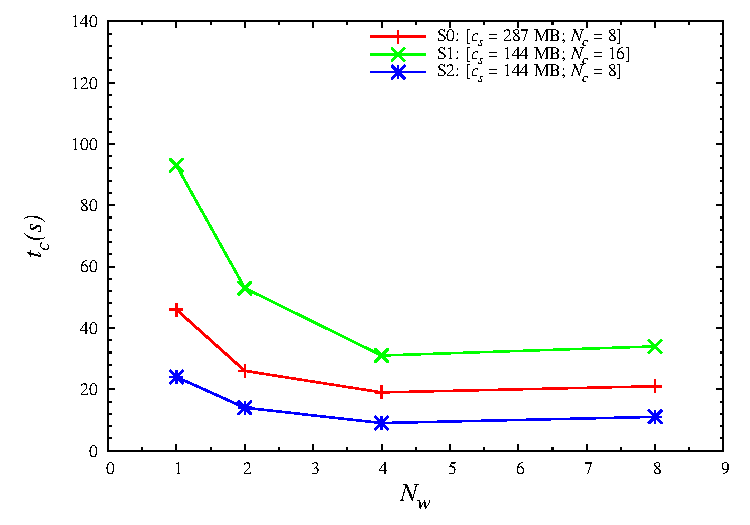
\includegraphics[scale=0.48]{data/graphs/LocalFigure}
\label{Fig:ExpIConventionalLocal:a}
}
\subfigure[$c_s=\mbox{287MB}$, GridFTP case]{
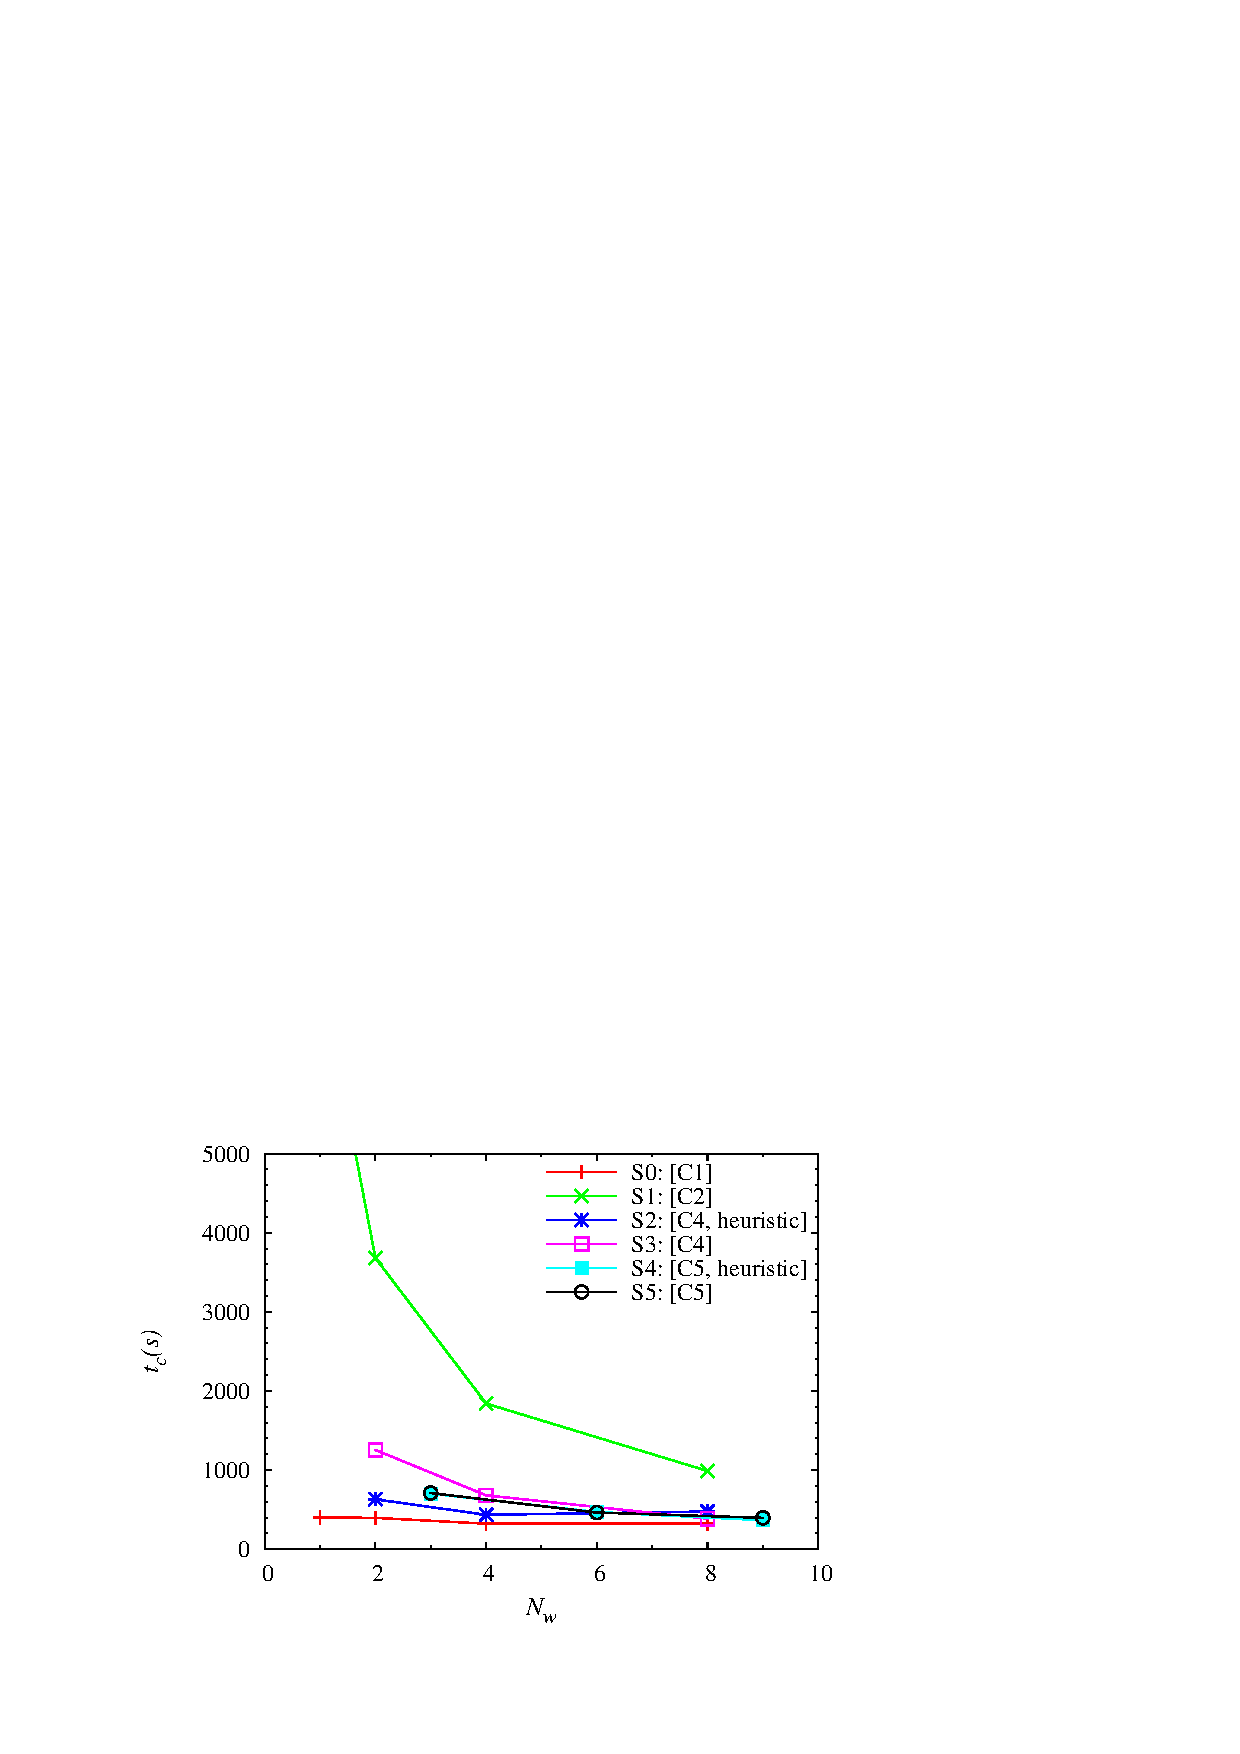
\includegraphics[scale=0.48]{data/graphs/ConventionalandIntelligent}
\label{Fig:ExpIConventionalLocal:b}
}
\caption{GridFTP vs. local run. We plot the time to
completion $t_c$ vs. the number of workers $N_w$. Note the scale, the
local case took less $t_c$ than the GridFTP case. In Fig.
\ref{Fig:ExpIConventionalLocal:a}, we note that by doubling the data set
size we doubled $t_c$ (S2 vs. S0), and that we created an overhead in S1 (vs. S2) by
increasing $t_x$ as a result of having more files. In Fig.
\ref{Fig:ExpIConventionalLocal:b}, the two-machine configurations took
more time than using a single machine. As expected, computing in one
machine, while having the data stored in another ($t_c=7360s$ for $N_w=1$ in S1 -- not pictured), took longer
compared to having some data stored in the resource performing
computations (S3). For up to 8 workers, $t_c$ decreased as $N_w$
increased, with the exception of a single machine where we reached an
I/O bound. Here, we also compare the GridFTP and the heuristic
approaches for two and three machines (Sec. \ref{Sec:Heuristic}). For
the two-machine case, we observed a performance improvement by using our
heuristic approach (S2 vs. S3). However, with more resources involved,
our heuristic system did not improve $t_c$ (S4 vs. S5).}
\label{Fig:ExpIConventionalLocal}
\end{center}
\vspace{-0.3cm}
\end{figure}

%%Figure was in the the section below
%\begin{figure}[!ht]
%\begin{center}
 %  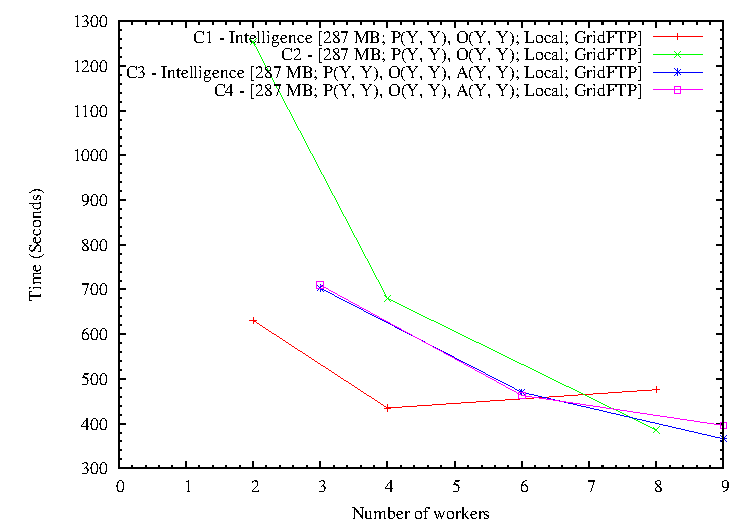
\includegraphics[scale=0.5] {data/graphs/IntelligentFigure}
%\end{center}
%\caption{\textit{$(c_s, N_c, f\!s, m)=(\mbox{287 MB, 8, local, gridFTP})$.
%%We compare the gridFTP and the intelligent approaches, for two and three
%%machines. In all cases, data was spread across all the resources For
%%the two-machine case, we observed a performance improvement by using our
%%intelligent approach. However, with more resources involved, our
%%intelligent system did not improve $t_c$.}}
%%\label{Fig:IntelligentExp}
%%\end{figure}


%%\vspace{-0.2in}

%Bety's graph goes here
% \jhanote{We need data for compute (comparison) and I/O (only) for
% different data-set sizes}

\vspace{-0.3cm}

%Staging experiment
\subsection{Experiment II: Heuristic Based System}\label{Sec:Heuristic}
The second experiment is similar to the first, except the All-Pairs
application is aware of the data location before determining whether or
not to assign a certain set of data-dependent computation to an idle
worker. Inspired by earlier work~\citep{netperf}, this version of the
application performs an extra step during application startup that
approximates the performance of the network by pinging the hosts that
may be either a computational resource or a data store. This information
is then assembled into a graph data structure. This graph is utilised at
runtime when the application needs to map an idle worker to an
unprocessed set of pairs defined in the XML file. This changes the
first-available computational resource assignment mechanism described in
the first experiment to a heuristic based system. Though ping is not
very sophisticated in terms of describing a network's behavior, it is a
first-approximation to a performance aware data-placement strategy. We
also experimented with the netperf application \citep{netperf_web} as a
method to describe a network's behavior, but since we were working with
such a static set of resources (LONI), the same data graph was generated
as with ping. The netperf-based heuristic system added approximately 8
seconds per resource of overhead due to the nature of the network
evaluation, but yielded no benefit.  Netperf has the advantage of being
able to determine throughput and bandwidth over multiple protocols.
These approaches know where the files are located and their distance to
available computational resources, thus allowing more intelligent
decisions when mapping a set of pairs to a computational resource. An
even more involved approach would be to manage locations of files
dynamically at run-time depending on usage patterns. We leave this
approach to future research. 
%Figure 2

The overhead of heuristics includes the time spent pinging hosts and
building the graph data structure. The total time spent for this
overhead was negligible at approximately two seconds per application
run. In figure \ref{Fig:ExpIConventionalLocal:b}, we see we achieved a
reduction in time to completion due to the use of heuristics. However,
when the same tests were performed utilising three resources instead of
two, the heuristic seemed to offer no significant reduction. The
explanation that we propose for this, is that the sets of pairs defined
in the configuration file at application start were geographically
equally dispersed throughout the network. Essentially, each set of pairs
had approximately the same cost calculated by using the graph data
structure. Each set of pairs would take the same time to compute using
any computational resource.

\vspace{-0.3cm}

\subsection{Experiment III: CloudStore}\label{Sec:CloudStoreExp}
The third experiment provides information into CloudStore's performance
in handling data locality issues. The same All-Pairs application as in
Experiments I and II is used, except all data is stored on the
distributed filesystem CloudStore under various configurations. Some
variables of importance include number of data servers that store data,
replication value for data in these data servers, and as above,
placement and number of computational resources. All read and writes
also utilise the distributed filesystem. Again, for our first set of
results, we don't add our comparison function, giving us
$t_{compute}=0$.
%Figure 3
\begin{figure}
\begin{center}
\subfigure[One and two machines]
{
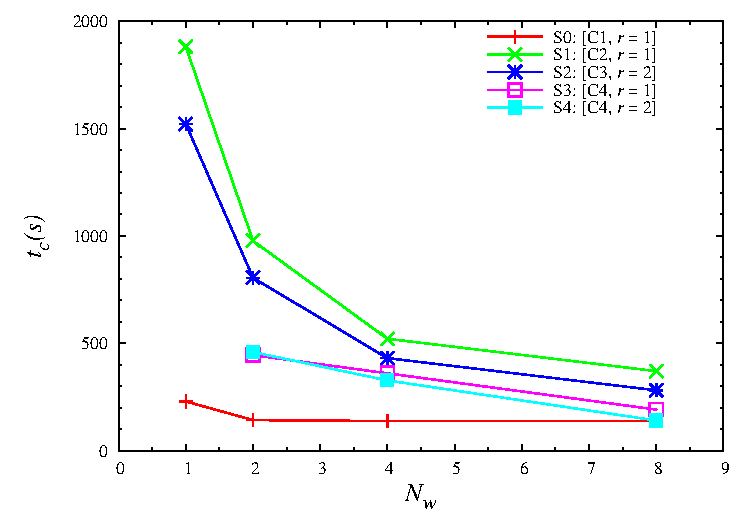
\includegraphics[scale=0.48]  {data/graphs/CloudStoreFigure}
\label{Fig:experiment3:a}
}
\subfigure[Three machines]
{
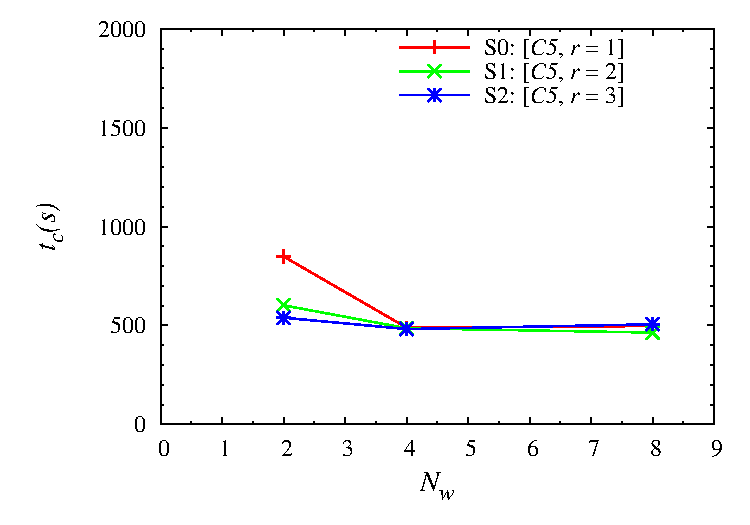
\includegraphics[scale=0.48] {data/graphs/CloudStore3Mach}
\label{Fig:experiment3:b}
}
\caption{(287MB,  CloudStore).
The figure on the left demonstrates All-Pairs' performance
with CloudStore locally and on two different machines. The figure on the
right demonstrates how this scales to three machines, for degree of
replication $r=1,2,\mbox{and } 3$. CloudStore performed better than our
local and heuristic-based approaches (see Fig.
\ref{Fig:ExpIConventionalLocal}). Again,
having data in the resource with the workload decreased $t_c$. When data
was spread across all the computational resources, having a degree of
replication $r = 1, 2, \mbox{or } 3$ did not significantly decrease
$t_c$, except to the case of three machines and 2 workers.}
%\jhanote{This caption needs attention}}
\label{Fig:experiment3}
\end{center}
\vspace{-0.3cm}
\end{figure}

As done above for the first experiment, we attempted to capture how
compute time scales under these configurations, see figure
\ref{Fig:experiment3}. Accessing data remotely adversely affected the
performance. We can see that computing in one resource while the data
was on another (S1) took the greatest amount of time. Having data in the
resource that was computing helped performance (S2, S3, S4). The number
of machines to which workload was assigned was also important. Placing
workload on two machines also decreased $t_c$ (S2 vs. S3). We varied the
degree of replication for the \textit{C4} and \textit{C5} configurations, i.e., for
the cases of two and three machines, where all the resources had
workload assigned and data stored. With a replication degree larger than
one, data was almost certainly co-located with the computational
resource. For \textit{C4}, having $r = 2$ improved $t_c$, but not considerably.
For \textit{C5}, different degrees of replication only made a difference in the
case of two workers.

We then added the actual genome comparison function and we compared it
to the base case where we did not include the function. We define $\Delta t_c$
which is the time difference between these two cases. In figure
\ref{Fig:experiment4}, we see that the time taken to do the genome
comparison was relatively small compared to the set up time, transfer,
and I/O time added together. The fact that $\Delta t_c$ for a given
$N_w$ was not the same for most of configurations, shows that there was
still an overhead; $t_x$ and $t_{I/O}$ were not the same at the
times we ran our All-Pairs framework for both cases.
%Figure 4

\begin{figure}
\begin{center}
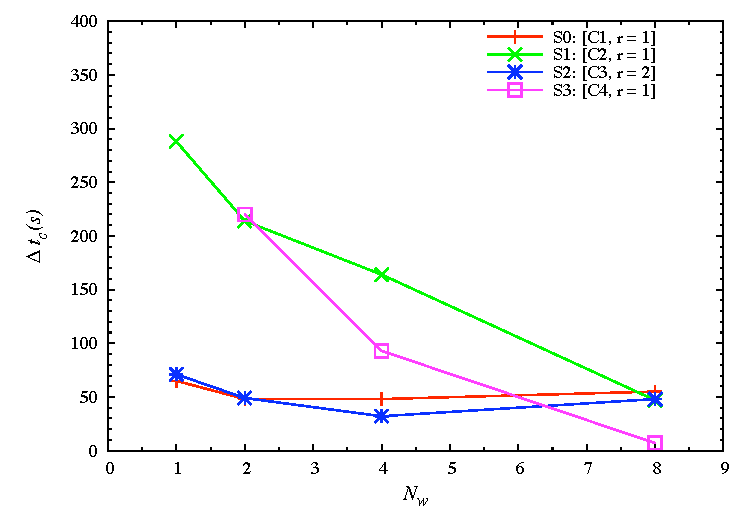
\includegraphics[scale=0.5]{data/graphs/CloudStoreComputeMinusNoCompute144}
\caption{(144MB, CloudStore). Comparison of CloudStore using the All-Pairs application with
and without actual computation. $\Delta t_c$ is defined as the time it
takes to run our framework where we include our genome comparison
function, minus the time it takes to run it when we don't include the
comparison function. For the case of $c_s=144\mbox{MB}$, our genome function
took about two orders of magnitude less than $t_x$ and $t_{I/O}$
combined. $\Delta t_c$ at a given $N_w$ differed for most of our
configurations, showing an overhead, probably caused by different
network conditions at the times our runs were performed.}
\label{Fig:experiment4}
\end{center}
\vspace{-0.5cm}
\end{figure}

We also compared the results with no comparison function
($t_{compute}=0$) for two different data set sizes, one with $c_s =
287\mbox{MB}$, and the other one with half the size, $c_s = 144\mbox{MB}$ (rounded
value). Both used CloudStore, and have eight assignments. We defined two
quantities, $\Delta t_c^d = t_c(287\mbox{MB}) - t_c(144\mbox{MB})$, and
$t_{OH} = 2 \times t_c(144\mbox{MB}) - t_c(287\mbox{MB})$. Figure
\ref{Fig:CloudStore287minus144} shows that there are multiple factors
that can alter $t_c$. Some of the factors are network conditions, I/O
time, as well as transferring time that can be size dependent, disk seek
time, etc. In figure \ref{Fig:CloudStore287minus144:a}, we see that the
difference did not scale linearly with the number of workers. It is
worth noticing that $\Delta t_c$ was almost zero (and negative) for
eight workers when all the resources had workload and data stored (S3);
this is, it took about 10 seconds less for a 2.3GB set vs. a 1.15GB
set. Figure \ref{Fig:CloudStore287minus144:b} shows that for most of our
cases, there was an overhead which decreased with the number of workers.
It also shows us that the remote data configuration was the one with the
most overhead. Moreover, our S3 case seemed to use a ``non scalable''
infrastructure, as the overhead increased with eight workers.

\begin{figure}
\begin{center}
\subfigure[$\Delta t_c^d (= t_c(287\mbox{MB}) - t_c(144\mbox{MB})) \times N_w$]
{
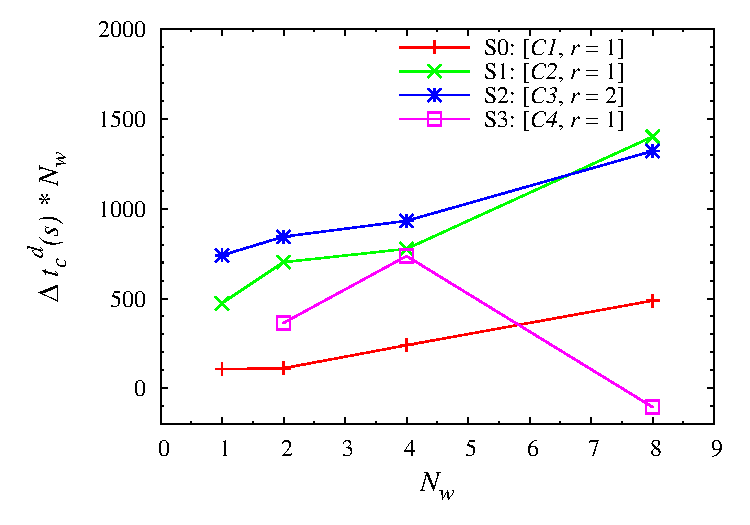
\includegraphics[scale=0.48]{data/graphs/CloudStoreNoCompute_287Minus144TimesNw}
\label{Fig:CloudStore287minus144:a}
}
\subfigure[$t_{OH}=2 \times t_c(144\mbox{MB})-t_c( 287\mbox{MB})$]
{
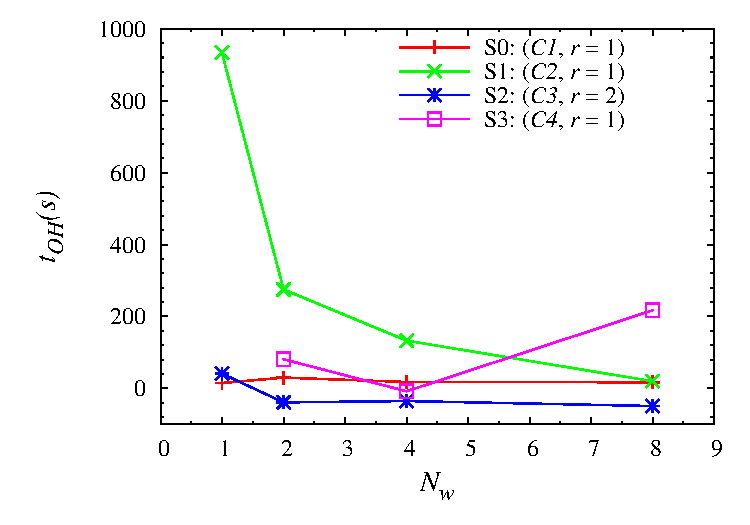
\includegraphics[scale=0.48]{data/graphs/CloudStoreNoCompute_287Minus144CommonTime}
\label{Fig:CloudStore287minus144:b}
}
%%\subfigure[$\Delta t_c$]
%%{
%%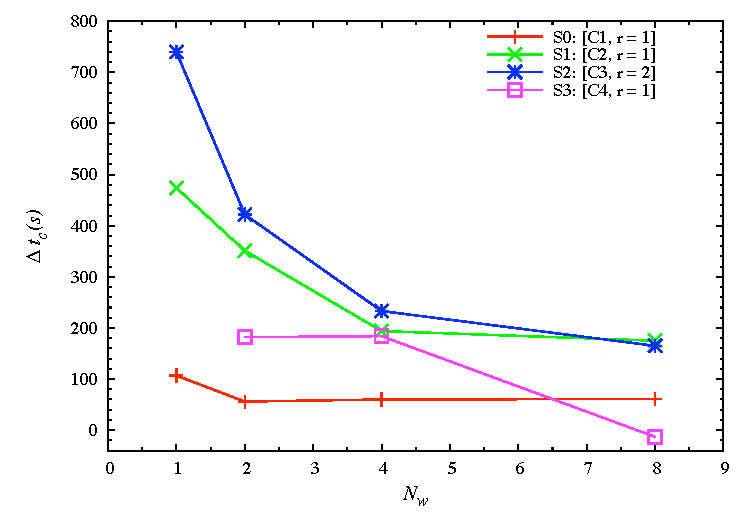
\includegraphics[scale=0.5]{data/graphs/CloudStoreNoCompute_287Minus144}
%%\label{Fig:CloudStore287minus144:c}
%%}
\caption{(CloudStore). Here
we define two quantities, $\Delta t_c^d$, and $t_{OH}$. $\Delta t_c^d$
is the difference between $t_c$ found for data set sizes 1.15GB and
2.3GB, this is, for chunk sizes $c_s = 144\mbox{MB and } 287\mbox{MB}$.
$t_{OH}$ is the overhead time of working with chunks of 287MB in size
vs. 144MB chunks twice. In figure \ref{Fig:CloudStore287minus144:a} we
see that the difference $\Delta t_c^d$ decreased with increasing number of workers, but did
not scale inversely proportional with $N_w$; this would be indicated by horizontal lines. In figure
\ref{Fig:CloudStore287minus144:b}, we see that S1 (remote data)
was the one with the most overhead.}
\label{Fig:CloudStore287minus144}
\end{center}
\vspace{-0.4cm}
\end{figure}

We compared the lowest times for both our heuristic approach and
CloudStore as a function of the number of resources $N_r$ in figure
\ref{Fig:CloudStoreVsGridFTP} (left subfigure). CloudStore performed better for one and
two machines, but not for three resources, when CloudStore decreased its
performance. The lowest times of our heuristic approach were about the
same for $N_r=1,2,3$. In figure \ref{Fig:CloudStoreVsGridFTP} (right subfigure) we
plotted our completion time as a function of the number of workers for
three resources. All the resources had workload assigned and data
stored. CloudStore's performance did not vary significantly with the
number of workers, while our heuristic approach performed better as we
increased the number of resources from one to three.

\begin{figure}
\begin{center}
\subfigure
{
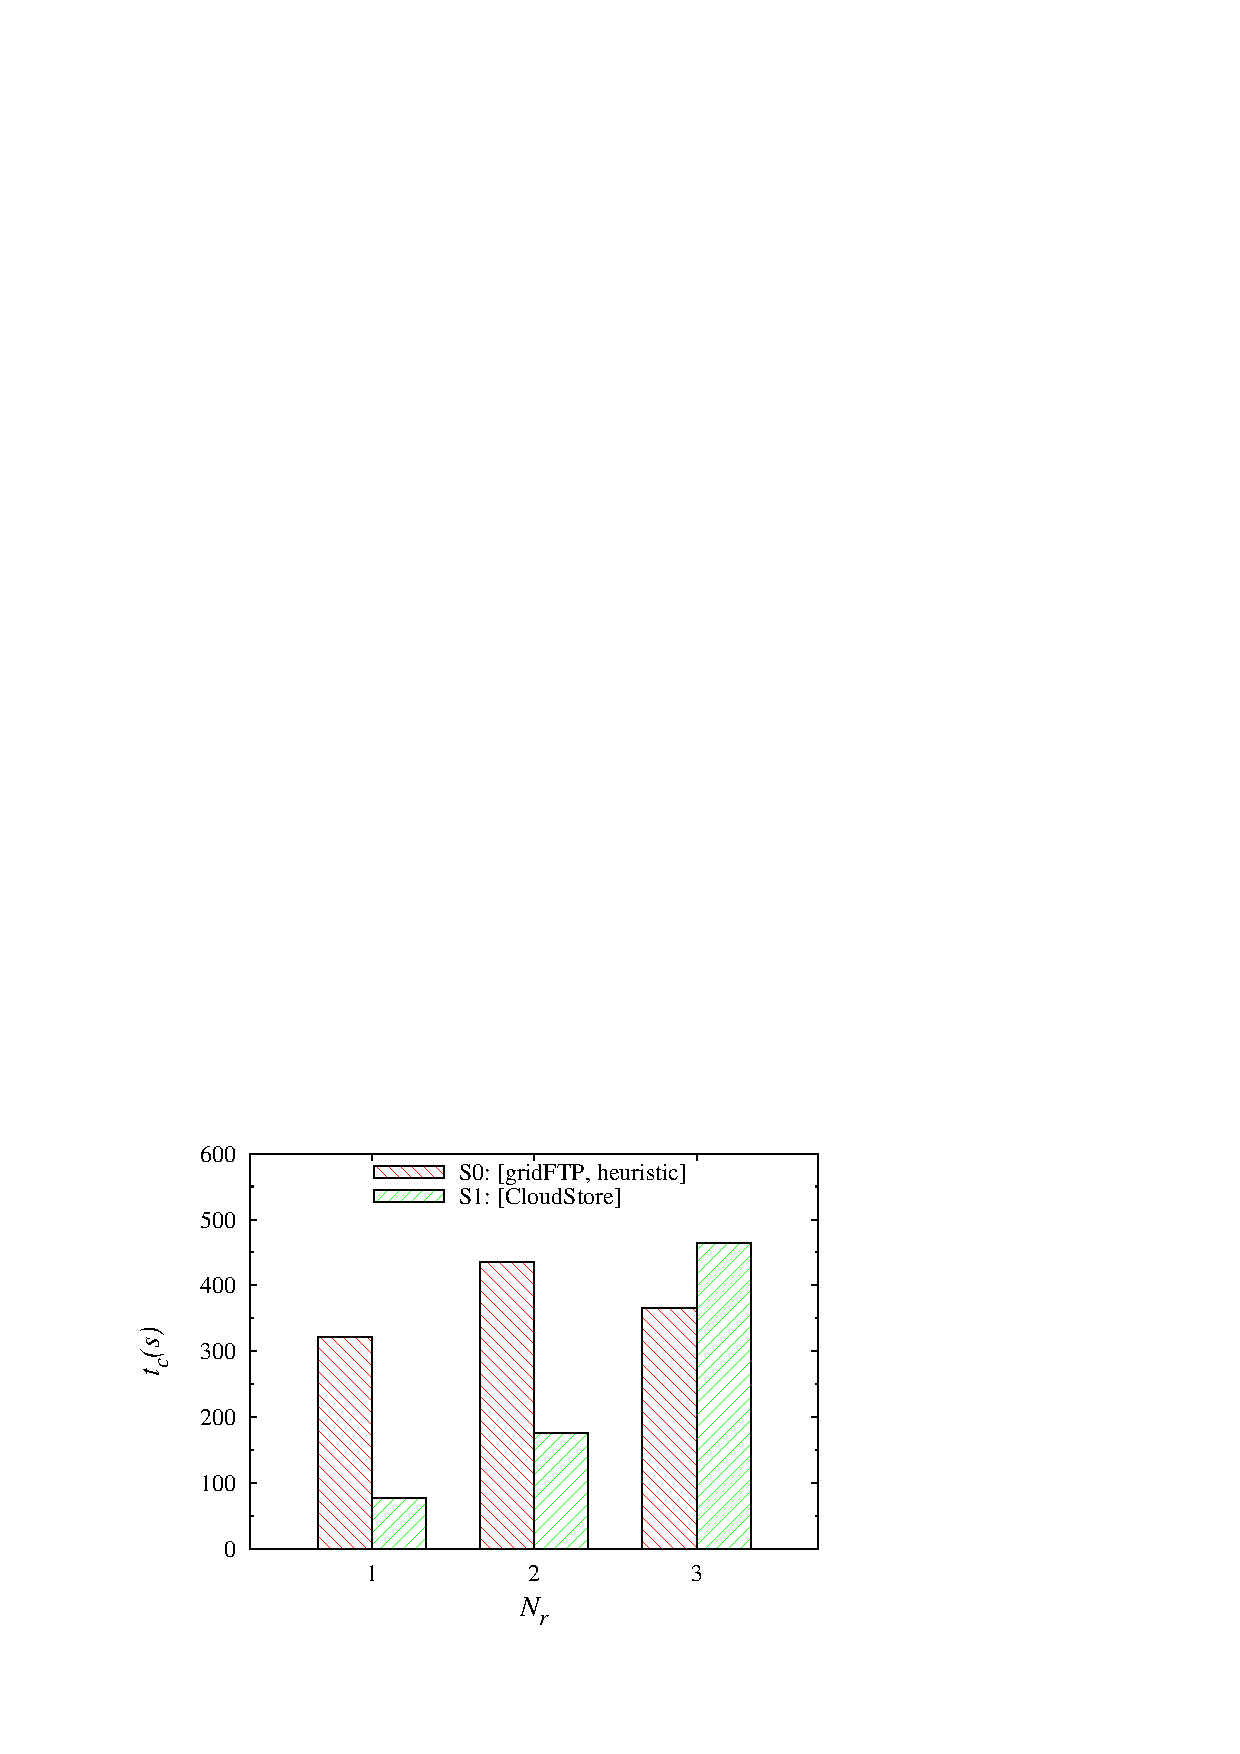
\includegraphics[scale=0.48]{data/graphs/NumberResourcesFigure_histogram}
\label{Fig:CloudStoreVsGridFTP:a}
}
\subfigure
{
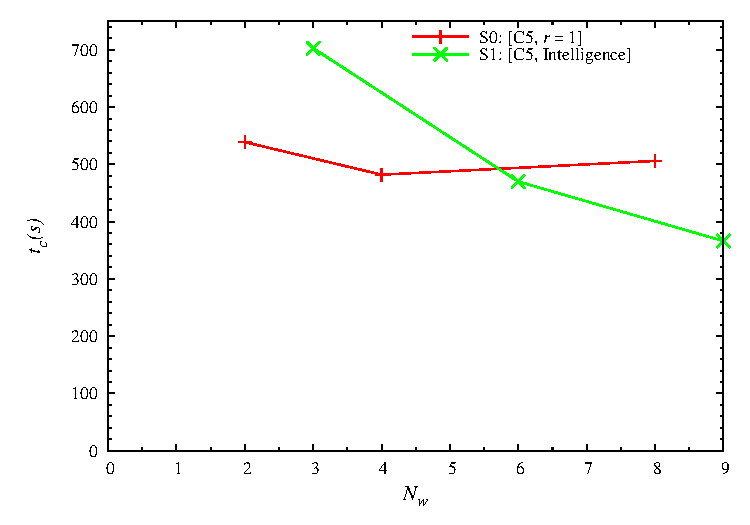
\includegraphics[scale=0.48]{data/graphs/CloudStoreVsGridFTPFigure}
\label{Fig:CloudStoreVsGridFTP:b}
}
\caption{(287MB). [Left] The figure
 shows the lowest times we achieved for a given number of resources
 $(N_{r})$. These lowest times did not vary much for our heuristic-based 
 method, while CloudStore decreased its performance by adding number of
 resources (up to three). [Right] The figure
 demonstrates performance with three resources for both GridFTP and
 CloudStore. The three resources computed and had data stored.
 Performance using CloudStore remained about constant for two, four, and
 eight workers, while our heuristic approach improved its performance
 with the number of workers.}
\label{Fig:CloudStoreVsGridFTP}
\end{center}
\vspace{-0.4cm}
\end{figure}

%\section{Analysis}

Overall, the use of CloudStore decreases the time to completion
($t_c$) compared to the intelligent and the local approaches. Our
simple intelligent approach did not performed as well as CloudStore, but
works better than the local tests. For the parameters we used, the
introduction of more workers, up to 8 in our case, decreases the time of
completion; however, for the case of a single machine performing as both
master and workers, we hit an I/O bound, probably caused by the network.
For all of our approaches, GridFTP, Intelligent, and CloudStore, we find
the time to completion for three cases: a single machine is the master
and the workers, one machine does the computing while another has the
data stored, and the case when we spread the data into both machines,
while both of them compute.  In all of our three approaches, the case of
a single machine, shows the least $t_c$. In the case of two machines,
having the data in one, and computing in the other one, increases the
time to completion. By splitting the data in both of the machines, and
computing in both, we decrease $t_c$. We then added another case, all
the data in each of machines, and computing in both. This decreases the
time even further, but not to the point of the local computations;
perhaps, all the approaches are not guaranteed to use the data in the
machine the job is being run, even thought the data is in both machines.

???For our three cases,  $t_c$ may be bounded, and decrease to $t_c$(single machine) as  the number of workers ($N_w$) increases, up to a critical $N_w$, after which $T_c$ will increase due to worker coordination overhead.




\vspace{-0.3cm}

\section{Conclusions and Future Work}

% \section{Analysis} % In addition, we did not utilise
% more than 3 distributed resources, because the Globus toolkit was installed in
% only three machines. 

We set out to understand the factors that influence the performance of
a representative data-intensive application, and to understand their
interplay. We also aimed to demonstrate how the SAGA approach enables
data-intensive applications to be extensible and interoperable over a
range of infrastructure.  This capability enabled us to compare and
contrast two different approaches -- simple application-level data
placement heuristics versus distributed file systems -- for executing
distributed data-intensive applications. It should be noted that 
utilising SAGA to access CloudStore-based and GridFTP-based files
introduced a small but negligible overhead.

For the volume of data we worked with in the first set of experiments,
the local configuration (\textit{C1}) took the least time to completion $t_c$
as a function of the number of workers $N_w$. However, this will not
necessarily be the case as the volume of data is largely increased
(which we anticipate to be tens of GB of data).  The remote
configuration (\textit{C2}) showed the highest time to completion, while
$t_c$ decreased for the mixed configuration (\textit{C3}). Using
configuration \textit{C4} decreased the time even further, but not to the
point of \textit{C1}. $t_c$ appears to be bounded by $t_c(\mbox{local})$,
where we exhausted the I/O bandwidth.  In general, $t_c$ decreased as
we added more workers, but it is expected that after a critical value
of $N_w$ ($N^c_w$), $t_c$ will increase due to overhead of
coordinating workers.

The second experiment implements a simple heuristic for efficient data
and work resource assignments.  This staging phase only required
performing pings, not data transfer trials or reliability tests.  The
staging phase is worth the time required to build a network graph, as
it improved upon the results of the naive baseline performance
experiment. Our experiments scaled to three distinct resources not due
to any fundamental scalability limitation in our approach, but due to
the inability to find more than three similar resources.
 
Overall, the use of CloudStore lowers $t_c$ compared to the
heuristic and the GridFTP approaches. Our simple heuristic 
approach did not perform as well as CloudStore for one and two
machines, but performed better than a naive use of GridFTP.  For three
machines, the relative performance of CloudStore and the heuristic
approach depended upon the $N_w$.  Our results for three resources
showed that an heuristics-based use of GridFTP continued to experience
improvements in performance as the number of resources increased, while
CloudStore leveled off.  

We will extend this work to understand performance over a wider range
of infrastructure (DFS, distributed coordination and sharing
infrastructure such as BigTable, etc.) and different data-access
patterns, but also to explore correlations in data/file access.  Such
correlation in data-access has been observed elsewhere
(\cite{filecule}); devising specific abstractions to support such
correlated access and ``aggregation of files'' could enhance
performance for a broad range of data-intensive applications and would
be be both interesting and rewarding.

{\bf Acknowledgment:} Important funding for SAGA has been provided by
the UK EPSRC grant number GR/D0766171/1 (via OMII-UK), HPCOPS
NSF-OCI 0710874, and CyberTools NSF/LEQSF(2007-10)-CyberRII-01.
 SJ acknowledges the e-Science Institute, Edinburgh
for supporting the research theme, ``Distributed Programming
Abstractions'' and theme members for shaping many important ideas. BRM
is supported by LONI Institute, grant no. \
LEQSF(2007-12)-ENH-PKSFI-PRS-01. This work has also been made possible
thanks to the internal resources of the Center for Computation \&
Technology at Louisiana State University and computer resources
provided by LONI.

\vspace{-0.4cm}

% Attempting to determine if analogous abstractions could enhance
% performance for the All-Pair application could be interesting. In a
% DFS, however, if the data store is also capable of data processing,
% then a DFS has the information available to place commonly used files
% together on machines needing them for work; in essence, the DFS is
% capable of finding these groups for the developer. The fault
% tolerance, for which DFS are already well renowned for, also has added
% benefits to grid application developers in terms of performance.  The
% distributed application does not have to be aware of where data has
% been copied to previously when assigning work; the DFS uses the best
% replica when data is being accessed.

%\bibliographystyle{IEEEtran}
\bibliographystyle{kluwer} 
\bibliography{data_intensive_paper}
\end{document}

%Therefore, we introduce the idea of network-closeness. A network-close
%data-set takes a small amount of time to transfer to the work location.
%A network-far data-set is just the opposite. A network-far data-set
%takes a long time to transfer to the work location. If there is an
%unprocessed data-set collocated or network-close with the job, then the
%assignment of that worker to that data-set would have benefits. If there
%is no unprocessed data-set that is network-close to the job, still we
%assign data that may be network-far, in case the network-close job
%failed or there is no available jobs network-close to the data-set.

%There are at least two types of data-intensive applications: the first
%where the actual data generated is large; the second type is where the
%data generated is small, but the volume of data on which computation
%occurs is very large. The application we used, has relatively small
%input and relatively small output, but the manner of processing causes
%many data reads. This type of application can be classified as having
%a large data throughput. \jhanote{Can you elaborate on different
%types of data-intensive applications? What kind is an ImageMagic
%based application?}

% \jhanote{Compact. Simplify. Possibly move parts to later section; not
%  in introduction} Distributed filesystems (DFS) have come of age,
% with multiple open-source, reliant file-systems now available. DFS are
% useful and effective tools to consider for data-intensive scientific
% applications. A DFS controls the data placement and provides a
% uniform interface for accessing files on multiple hosts. Thus it is
% worth considering DFS as a viable infrastructure. But as the
% underlying algorithms, scheduling strategies and implementations vary
% greatly between different infrastructure, it is difficult to estimate
% {\it a priori} the application-level performance on a given DFS.
% .... Frequently, there is more than one copy of the input data for
% fault-tolerance reasons, consequently, the added issue of deciding
% between the two or more replicas becomes relevant. While a DFS
% removes the responsibility of replica management and data server
% placement, the abstraction often increases the difficulty in
% determining where in the DFS the data is being stored. This puts
% pressure on a DFS's protocols and internal algorithms to perform
% well. Despite this, the DFS replication may alleviate this issue by
% placing replicas in locations where computational resources reside. A
% downfall of DFS is the inability to make the decision of whether to
% move the input data, or the computational workload. It can only focus
% on minimizing poor data management. The most common parameters in
% determining the performance of using a DFS are the performance
% overhead compared to a normal local filesystem, number of replicas of
% each datum/file, and the number of servers. Our intelligent framework
% method differs from a DFS in that it determines where data is and
% where the work should go. Determining data location can be as simple
% as looking at the IP address of the worker and seeing geographically
% where it is located, or as complicated as using network analyses tools
% to determine the optimal data transfer minimization time. For this
% method, we use gridFTP\jhanote{place proper citation for gridftp}, a
% tool that is used to transfer files across machines in a grid. It is
% specifically designed for high-bandwidth networks.
 
% \section{Introduction} Data-intensive computing is a fast growing area
% of computer science. A good example of this is Google, which processes
% around 20 petabytes of data per day ~\citep{google}, and trends show
% continuing growth. It has become very important that a distributed
% application developer takes precautions when placing, scheduling, and
% managing large volumes of data. Careless placement can adversely affect
% system performance greatly. It is decisive then to determine whether to
% move input data to the computational resource, or the computational
% workload to the input data. There are two ways to handle this issue,
% with distributed filesystems, which focus on data placement, or with the
% use of an intelligent framework, which focuses on worker placement. 

% \jhanote{refine} Different metrics of concern for parallel
% vs. distributed data (I/O).  I/O typically dominated by Bandwidth for
% Cluster/Parallel systems, I/O dominated by latency. The challenge in
% load balancing for the former is often disc or bus-limited at the
% hardware level, while at the software/application level the challenge
% is to increase concurrent I/O with computation. For distributed
% systems and applications the challenge is to find an optimal
% distribution strategy that takes into account the ratio of
% computation workload to data distribution.  Data privacy, security and
% access policy is a crucial non-technical issue for distributed
% applications.  
% Distributed filesystems (DFS), motivated in part by developments in
% cloud computing, are useful and effective tools to consider for
% data-intensive scientific applications. A DFS controls the data
% placement and provides a uniform interface for accessing files on
% multiple hosts. Frequently, there is more than one copy of the input
% data for fault-tolerance reasons, consequently, the added issue of
% deciding between the two or more replicas becomes relevant. While a DFS
% removes the responsibility of replica management and data server
% placement, the abstraction often increases the difficulty in determining
% where in the DFS the data is being stored. This puts pressure on a
% DFS's protocols and internal algorithms to perform well. Despite this,
% the DFS replication may alleviate this issue by placing replicas in
% locations where computational resources reside. A downfall of DFS is
% the inability to make the decision of whether to move the input data, or
% the computational workload. It can only focus on minimizing poor data
% management. The most common parameters in determining the performance of
% using a DFS are the performance overhead compared to a normal local
% filesystem, number of replicas of each datum/file, and the number of
% servers. In our experiments, we use the stable open source distributed
% filesystem CloudStore (formerly KFS), which is written in C++ released
% under the Apache License Version 2.0. It is inspired by the highly
% successful Google Filesystem, GFS ~\citep{cloudstore_web}, which is
% closed source and unavailable for research. CloudStore was chosen for
% its high performance focus, C++ implementation, and its source code
% availability. It also provides a means to automatically replicate data
% on different hosts to provide efficient data access and fault tolerance. 

% Our intelligent framework method differs from a DFS in that it
% determines where data is and where the work should go. 
% Determining data location can be as simple as
% looking at the IP address of the worker and seeing geographically where
% it is located, or as complicated as using network analyses tools to
% determine the optimal data transfer minimization time. 
% For this method, we use gridFTP, a tool that is used to transfer
% files across machines in a grid. It is
% specifically designed for high-bandwidth networks. GridFTP is provided by
% the Globus Toolkit, an open source software toolkit
% released under the Apache License version 2.0. Globus provides tools used
% to create and manage grid infrastructures. 

% In this paper, we provide some initial approaches to answer ``To
% distribute or not to distribute data, is the question''. Our research
% focuses on understanding the performance trade-offs of a DFS compared to
% ''regular'' distribution and placement techniques, as well as more
% advanced intelligent distribution methods and finding how they handle
% different data-sets and what the performance patterns are. This paper
% also aims to determine how sensitive the performance is in the context
% of a real data-intensive distributed applications.
